\section{Correctness checks and controlled measurements}
\label{sec:experiments}

The experiments serve three purposes: detect implementation errors against
independent calculations, identify the source of an improvement, and find
conditions under which an improvement fails to help. They do not fit an
asymptotic exponent to a small sample and do not infer a worst-case theorem
from fast synthetic instances.

\subsection{Environment, timing scope, and censoring}

The principal runs use Python 3.12.14 on Linux x86-64 with glibc 2.39.
Independent geometric and polynomial checks use Regina distribution 7.4.1,
whose engine version string is 7.4 \cite{regina}. The package records full
runtime strings and source SHA-256 hashes. This is a shared execution
environment, without a claim of dedicated CPU isolation. Small differences
in sub-millisecond medians should be interpreted accordingly.

The tensor comparison uses seven measured rounds and one excluded warmup
per case and arm. Within each round it shuffles six arms using seed 2645:
faithful Potts, a second identical faithful control, certified Laurent tensor,
certified global-shift integer tensor, certified valuation-normalized integer
tensor, and an ordinary-order integer tensor. Every query starts with a fresh
validated diagram, computes the complete polynomial, and includes order
preparation. The allowance is 4,096 states, 200,000 transitions, and two
seconds per query. The ordinary-order arm is an ordering ablation and has no
universal width promise.

The overlap comparison uses five measured shuffled rounds, one excluded
warmup, and seed 3110. It runs the archived helper from the pinned revision,
an A/A repeat, and the optional helper in a common harness. Local timings
include grammar construction, the preceding whole-donor probe, the cyclic
query, and checked application. The local allowance is two million charged
work units and 100,000 nodes. Whole recognition timings include fresh input
validation and independent certificate replay. The exact benchmark options
and every raw sample are retained.

An exhausted allowance is recorded as \status{LIMIT}, never as a completed
negative query. It has no completed-query speedup ratio. A shorter time to
hit a limit can be worse performance, because it has produced no answer.
Likewise, an earlier but smaller greedy move is not interchangeable with a
maximal-gain move merely because both shorten a relator.

\subsection{Tensor correctness and full-polynomial timings}

The independent tensor audit performs 420 full-polynomial comparisons for
each of the three arithmetic modes, for 1,260 comparisons in total. It also
enumerates 23,676 smoothing states and follows 71,860 oriented smoothing
circles independently; every absolute turn is four. The cases exercise
mirrors, row permutations, signed arc relabelings, supplied orders, different
outer faces, and replay of separator certificates. These totals count audit
operations, not 1,260 distinct knots.

A separate program imports each diagram into Regina with independently
checked component count and writhe. Regina's polynomial variable is
$\sqrt t$, so its even exponents are divided by two, without a mirror
inversion. It checks 35 base inputs and their mirrors in all three tensor
modes, giving 210 further complete coefficient comparisons. Named examples,
deterministic braid closures, weaving diagrams through 24 crossings, and the
two residual-twist witnesses of Section~\ref{sec:jones-status} are included.
The independent conversion uses a closed binomial formula for the latter
formal-coordinate check, rather than the baseline's recurrence.

The final six-arm timing run contains 630 measured queries: 588 complete
and 42 capped, plus 90 excluded warmups. Every completed polynomial agrees
across the applicable arms. Table~\ref{tab:tensor-times} reports the full
15-case corpus; the code and raw data specify every input diagram.

% Generated by reproduce/make_research_tables.py; edit the generator, not this file.
\begin{table}[H]
\centering\footnotesize
\setlength{\tabcolsep}{3pt}
\renewcommand{\arraystretch}{1.12}
\begin{tabular*}{\linewidth}{@{\extracolsep{\fill}}lrrrrrrr@{}}
\toprule
Case & $n$ & \shortstack{Faithful\\(ms)} & \shortstack{A/A\\(ms)} & \shortstack{Laurent\\(ms)} & \shortstack{Global\\integer (ms)} & \shortstack{Normalized\\integer (ms)} & \shortstack{Ordinary\\integer (ms)}\\
\midrule
Trefoil & 3 & 0.107 & 0.120 & 0.273 & 0.260 & 0.278 & 0.179\\
Conway & 11 & 0.425 & 0.403 & 1.512 & 1.232 & 1.347 & 0.758\\
Kinoshita--Terasaka & 11 & 0.396 & 0.417 & 1.508 & 1.234 & 1.322 & 0.776\\
Hard unknot & 8 & 0.229 & 0.227 & 0.602 & 0.586 & 0.593 & 0.447\\
Five-strand stress & 36 & 2.013 & 2.316 & 9.664 & 6.677 & 6.699 & 4.498\\
Weaving $q=5$ & 10 & 0.419 & 0.411 & 1.412 & 1.234 & 1.326 & 0.818\\
Weaving $q=13$ & 26 & 1.209 & 1.177 & 6.393 & 4.478 & 4.031 & 2.608\\
Weaving $q=17$ & 34 & 1.967 & 1.820 & 9.839 & 5.483 & 5.428 & 3.313\\
Tree, depth 6 & 126 & 8.066 & 7.824 & 25.659 & 37.402 & 24.664 & \textsf{LIMIT}\\
Tree, depth 7 & 254 & 67.007 & 64.860 & 72.620 & 242.443 & 68.276 & \textsf{LIMIT}\\
Grid $4\times4$ & 16 & 0.473 & 0.461 & 1.704 & 1.724 & 1.694 & 1.039\\
Grid $6\times6$ & 36 & 1.434 & 1.411 & 5.441 & 4.977 & 5.172 & 3.183\\
Grid $8\times8$ & 64 & 4.554 & 4.478 & 13.699 & 13.050 & 12.090 & 8.255\\
Grid $10\times10$ & 100 & 30.232 & 33.614 & 43.047 & 43.681 & 35.147 & 25.901\\
Shuffled $8\times8$ & 64 & 20.268 & 20.260 & \textsf{LIMIT} & \textsf{LIMIT} & \textsf{LIMIT} & \textsf{LIMIT}\\
\bottomrule
\end{tabular*}
\caption{Complete full-Jones queries: median milliseconds over 7 randomized paired rounds after 1 warmup round. A/A is an independently timed repeat of the faithful arm. Order construction and verification are included; the ordinary-integer arm omits the universal width certificate. \textsf{LIMIT} denotes a capped arm, not a completed-query runtime; no ratio is assigned to it. Per-query limits were 2 seconds, 4,096 states, and 200,000 transitions. These invariant-query measurements do not measure complete recognition.}
\label{tab:tensor-times}
\end{table}


The faithful implementation remains faster on most of these inputs. This
does not conflict with the improved universal bound: equality partitions
can collapse to very small tables on favorable actual diagrams. For example,
the recorded Conway calculation has five faithful states versus nineteen
binary tensor states; the favorable shading of the 254-crossing tree medial
has one faithful state versus 272 tensor states. A smaller asymptotic worst
case does not force a smaller table on every instance.

Within the tensor implementations, valuation-normalized integers improve
several cases. The median \emph{paired} Laurent/normalized ratios are 1.885
on the 34-crossing weaving case, 1.432 on the 36-crossing stress braid, 1.151
on the 100-crossing grid, and 1.072 on the 254-crossing tree medial. The
trefoil ratio is 0.994, providing no improvement. Paired ratios need not equal
ratios of the separately reported median times.

The global-shift arithmetic ablation reveals a specific avoidable cost.
On the 254-crossing tree medial it retains 130,177-bit scalars and takes
242.443 ms, whereas valuation normalization retains 1,536-bit mantissas and
takes 68.276 ms. Both compute the same exact polynomial, with the same
binary frontier method. Table~\ref{tab:tensor-precision} and
Figure~\ref{fig:tensor-precision} show the corresponding precision counts.

% Generated by reproduce/make_research_tables.py; edit the generator, not this file.
\begin{table}[H]
\centering\footnotesize
\setlength{\tabcolsep}{3pt}
\renewcommand{\arraystretch}{1.12}
\begin{tabular*}{\linewidth}{@{\extracolsep{\fill}}lrrrrr@{}}
\toprule
Case & $n$ & \shortstack{Faithful\\scalar bits} & \shortstack{Laurent\\coefficient bits} & \shortstack{Global\\integer bits} & \shortstack{Normalized\\mantissa bits}\\
\midrule
Tree, depth 6 & 126 & 63,757 & 2 & 32,321 & 768\\
Tree, depth 7 & 254 & 258,573 & 2 & 130,177 & 1,536\\
Grid $10\times10$ & 100 & 10,855 & 2 & 10,921 & 832\\
\bottomrule
\end{tabular*}
\caption{Maximum bit length of one stored scalar, Laurent coefficient, or normalized mantissa in completed queries from the final paired run. The values agree across all repeated samples. They are not total table-memory measurements: the normalized mode also stores a valuation, and every mode stores frontier keys and other metadata. The two integer tensor modes use the same exact polynomial model and certified order.}
\label{tab:tensor-precision}
\end{table}


\begin{figure}[H]
\centering
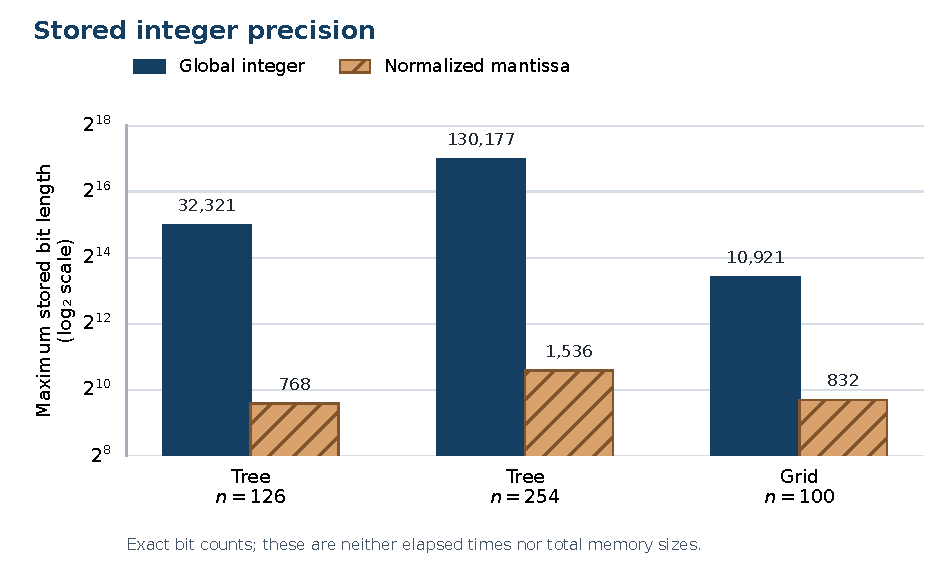
\includegraphics[width=0.92\linewidth]{figures/tensor_precision.pdf}
\caption{Retained scalar precision in the same exact tensor contraction,
with and without valuation normalization. The axis is logarithmic and the
labels give exact bit counts. This measures monomial-padding removal, not
an asymptotic running-time fit or a change in frontier width.}
\label{fig:tensor-precision}
\end{figure}

The ordering controls also matter. The certified tensor orders complete the
two large tree cases where ordinary-order integer tensors hit the state cap.
Conversely, every tensor mode hits the cap on the shuffled 64-crossing grid,
while faithful Potts completes. Thus the new backend adds a stronger exact
general bound and an alternative performance profile; it does not dominate
the existing backend on the supplied finite corpus.

\subsection{Cocycle seeds: exact objectives and genuine manifolds}

The cocycle data contain seven explicit product-solid-torus cases, a
one-vertex numerical limitation example, and two genuine finite knot
exteriors. The product construction triangulates $D^2\times S^1$ by
staircase tetrahedra. It starts with the primitive circle cocycle and adds
a large global vertex coboundary. Hence the huge initial weight represents
the same fixed primitive class; this deliberately isolates dependence on
binary height size.

% Generated by reproduce/make_research_tables.py; edit the generator, not this file.
\begin{table}[H]
\centering\footnotesize
\setlength{\tabcolsep}{3pt}
\renewcommand{\arraystretch}{1.12}
\begin{tabular*}{\linewidth}{@{\extracolsep{\fill}}rrrrrr@{}}
\toprule
$T$ & \shortstack{Height\\bits} & $\bits(D_0)$ & $D_\star$ & \shortstack{Optimizer\\(ms)} & \shortstack{Checker\\(ms)}\\
\midrule
9 & 1 & 2 & 3 & 0.812 & 0.125\\
9 & 20 & 23 & 3 & 0.657 & 0.111\\
9 & 260 & 263 & 3 & 1.035 & 0.134\\
9 & 4100 & 4103 & 3 & 1.163 & 0.128\\
24 & 20 & 25 & 3 & 3.599 & 0.250\\
48 & 20 & 26 & 3 & 15.221 & 0.498\\
96 & 20 & 27 & 3 & 46.796 & 0.954\\
\bottomrule
\end{tabular*}
\caption{All seven product-solid-torus cases. $T$ is the number of tetrahedra; $D_0$ and $D_\star$ are the initial and optimal numbers of normal discs. Height bits are measured from the supplied local heights, rather than inferred from a case-name parameter. Times are single recorded calls, not paired benchmark medians. Optimization includes its internal certificate check; the checker column measures an additional certificate and face-matching check. These cases verify binary-height handling and the fixed-family optimum; they do not establish an end-to-end recognition speedup.}
\label{tab:cocycle-times}
\end{table}


The largest-height nine-tetrahedron case starts with a disc count having
4,103 bits and returns a three-disc meridian seed. Its flow still takes
exactly nine augmentations. It therefore tests the absence of loops
proportional to numerical weight. The timings in this table are individual
recorded observations, not paired medians or a random-knot study. In the
one-vertex numerical case, the initial and optimized counts remain equal;
the optimizer correctly certifies that a common vertex shift changes no
span. No manifold is asserted for that arbitrary-height one-row example.

For a geometric test independent of the artificial large coboundaries, the
audit truncates two-tetrahedron ideal trefoil and figure-eight exteriors to
finite triangulations. Each has 56 tetrahedra and ten vertices. The existing
archive02 exact spanning-tree routine supplies a cocycle; rank one and a
coordinate gcd of one verify integral primitivity. The optimizer does not
choose a different homology class.

% Generated by reproduce/make_research_tables.py; edit the generator, not this file.
\begin{table}[H]
\centering\footnotesize
\setlength{\tabcolsep}{3pt}
\renewcommand{\arraystretch}{1.12}
\begin{tabular*}{\linewidth}{@{\extracolsep{\fill}}lrrrrrrr@{}}
\toprule
Knot exterior & $T$ & $|V|$ & $D_0$ & $D_\star$ & \shortstack{Optimizer\\(ms)} & $\chi$ & $b$\\
\midrule
Trefoil & 56 & 10 & 109 & 54 & 19.655 & -1 & 1\\
Figure-eight & 56 & 10 & 60 & 38 & 20.832 & -1 & 1\\
\bottomrule
\end{tabular*}
\caption{Two genuine finite knot exteriors obtained by truncating Regina's ideal examples. A primitive tree-gauge cocycle is optimized within its vertex-potential family. Regina independently verifies that each output is connected and orientable; $\chi$ and $b$ denote its Euler characteristic and boundary-component count. The single-call times include the triangulation adapter's seed construction and consistency checks, but exclude triangulation construction, cohomology preparation, and the independent Regina check. Disc-count optimality in this family does not assert genus minimality or incompressibility.}
\label{tab:cocycle-exteriors}
\end{table}


The disc counts fall from 109 to 54 and from 60 to 38. Regina independently
checks valid orientable finite manifolds and connected orientable surfaces
of Euler characteristic $-1$ with one boundary component. Exact gluings,
isomorphism signatures, cocycles, normal coordinates, and primal/dual
certificates are included in the JSON. Simplifying these exteriors first
produces one-vertex triangulations and removes this optimization freedom;
the choice to optimize the finite truncations is explicit.

Fifteen focused tests also compare small instances against exhaustive
primal searches and dual permutation oracles, exercise repeated vertices
and cancellation, reject corrupt certificates, handle 4,096-bit heights,
and check archive02 interoperability. The independently verified equality
of primal and dual objectives is the evidence of optimality. A decreased
disc count by itself is not evidence of faster hierarchy construction.

\subsection{Overlap measurements, controls, and unchanged corpus paths}

\begin{table}[H]
\centering\small
\begin{tabular}{@{}lrrrrr@{}}
\toprule
Family, $N=2^h$ & Old ms & A/A ms & Witness ms & Witness work & Nodes\\
\midrule
Prefix, $h=8$ & 174.971 & 161.297 & 0.551 & 708 & 64\\
Prefix, $h=32$ & LIMIT & LIMIT & 0.731 & 1,308 & 112\\
Prefix, $h=500$ & LIMIT & LIMIT & 5.220 & 13,008 & 1,048\\
Interior, $h=8$ & 201.398 & 159.737 & 0.503 & 962 & 76\\
Interior, $h=32$ & LIMIT & LIMIT & 1.239 & 1,898 & 148\\
Interior, $h=500$ & LIMIT & LIMIT & 8.100 & 20,150 & 1,552\\
Shared tail, $h=500$ & 7.012 & 5.772 & 6.916 & 12,939 & 1,042\\
Gain tradeoff & 0.240 & 0.231 & 0.190 & 488 & 43\\
\bottomrule
\end{tabular}
\caption{Five-round medians for complete local search and application.
The strict-majority family has the same final overlap and gain in each
successful arm. The gain-tradeoff row intentionally has different move
quality. LIMIT means exhaustion of two million charged work units.}
\label{tab:overlap-times}
\end{table}

On the $h=8$ prefix and interior cases, old charged work is respectively
245,591 and 319,306 units. The optional counts are 708 and 962. For larger
$h$, the old arms exceed the allowance, so no numerical speedup factor is
reported. The retained shared-tail control shows no convincing gain, as
predicted by the cyclic-factor analysis. In the no-majority $h=500$ control,
all arms exhaust in whole-donor search with zero witness-helper calls.

All 225 measured whole-knot queries retain identical certificate digests,
and none reaches the changed compressed LCS helper. The sums of medians for
fourteen smaller inputs are 140.334, 140.396, and 138.959 ms for old, A/A,
and optional arms. Gordian medians are 1.5253, 1.5104, and 1.4790 seconds.
These numbers support no knot-corpus speedup claim for the new helper.

The reachable Gordian residual produces the same first move, 142-move
certificate, and 4,280 allocated nodes in each arm. Charged work changes
only from 155,142 to 155,168. Its five-round medians, 69.55, 63.42, and
87.21 ms, fluctuate more than the small work difference would suggest and
show no stable improvement. The complete trace is supplied because it
validates the real certificate boundary, not because its timing favors the
new method.

\subsection{Maintained test inventory and the worker correction}

Final discovery contains 721 tests in 83 maintained modules. The recorded
validation covers this inventory through ordinary \code{unittest} module
runs, with Regina distribution 7.4.1 enabled and no skipped tests. Before
the worker repair, all 720 then-existing tests ran: 719 passed and the
unchanged large-input worker regression raised a timeout. That error
reproduced in isolation. It was a compatibility defect in partial-input
communication on the inspected Python 3.12.14 runtime, rather than evidence
of a mathematical failure in any of the three primitives.

Only \path{fastunknot/normal_surface.py} and its test module changed after
that comprehensive batch. The other 82 modules supply 712 passing tests;
the affected worker module subsequently passes all nine tests, including
one added cleanup regression. Thus the final coverage is
$712+9=721$ current tests. A further six-test public-integration rerun also
passes; those six belong to the retained 712 and are not counted twice.
The affected module is the only test module using the worker transport;
the cocycle adapter tests import Regina directly. No existing test's
deadline or expectation was relaxed. The complete accounting, final source
hashes and raw logs are in \path{validation/final-validation.json} and the
adjacent validation files.

An earlier single-process discovery attempt ended with exit code 1 after
14 passing lines, without a unittest summary or traceback. Its cause was
not established; the next test passed in isolation. This attempt is
preserved and classified as incomplete, separately from the comprehensive
module runs. We do not report a successful final single-process suite run.


The checks distinguish discovery from verification. Seed-certificate
verification runs without the flow solver. Group-certificate replay runs
without the producer. Tensor output is compared to both an independent
state-sum oracle and an external exact implementation. Resource tests ensure
that incomplete operations cannot publish a partial invariant or a false
decision. Those boundaries are more consequential than simply increasing
the number of test cases.

\subsection{Interpretation of the evidence}

The empirical conclusions are deliberately specific. The binary tensor
backend improves a proved repository asymptotic bound. Valuation normalization
removes measured arithmetic overhead within that backend. Cocycle flow
reduces a certified geometric objective on two actual knot exteriors and
handles huge binary heights without expansion. Threshold-first overlap
substantially accelerates a proved compressed stress family. None of these
observations demonstrates a quasi-polynomial growth law for complete
recognition, and the supplied negative controls identify concrete reasons
why such an inference would be invalid.
